\section{Static costing of threshold reforms}
\label{sec:static}

A static costing measures the first-order revenue effect of a reform by re-applying
the tax rule to a fixed firm population, with no behavioural response. Let firm $i$
have turnover $y_i$, calibrated net VAT liability $v_i = \tau(y_i - x_i)$
(Section~\ref{sec:data}), weight $w_i$, scope flag $s_i$ (one for firms in
the VAT net), data-year registration flag $q_i$, and baseline
voluntary-registration flag $r_i$ (one for firms registered with data-year
turnover at or below the data-year threshold $T_0$). A firm remits VAT only
once registered. Under a counterfactual threshold $T$ an in-scope firm is
registered when its data-year turnover is at or above $T$; a voluntary
registrant ($y_i<T_0$) is unchanged, since no threshold move changes its
obligation; out-of-scope firms never remit. Total VAT revenue at threshold $T$
is therefore
\[
  R(T) \;=\; \sum_i w_i\, v_i\, s_i \,
  \mathbf{1}\bigl\{\, y_i \ge T \;\lor\; r_i \,\bigr\},
\]
which reproduces the baseline registered set at $T=T_0$. Three conventions
follow and are worth stating. First, because voluntary registrants already
remit, a threshold cut credits only the liability of in-scope firms newly drawn
into the net: about 89\% of below-threshold frame enterprises are already
registered (Section~\ref{sec:data}), so the firms a cut mainly reaches are the
unregistered stratum. Second, a threshold rise releases every in-scope
registrant with data-year turnover in $[T_0,T)$: they no longer need to
register, which is the reading HMRC's costing uses; the statutory
deregistration threshold (\pounds2{,}000 below the registration threshold)
would keep an existing registrant in the top of the band in the net, and I
report that as a sensitivity. Third, the headline treats every released firm as
deregistering; the anchor comparison reports the voluntary-retention
sensitivity. Band membership is evaluated on \emph{data-year} turnover in every
fiscal year: a static cross-section has no growth process, and ageing the
near-threshold stock across the threshold by a uniform factor would treat
bunched firms as crossers, which they are not by construction
(Section~\ref{sec:bunching}). Liabilities are aged by a cumulative
nominal-growth factor---1.031, 1.052, 1.078, 1.110, and 1.142 for 2024--25 to
2028--29 relative to 2023--24 (the anchor runs on the 2023--24 vintage; the
sweep on the 2024--25 vintage, aged relative to its own data year); the
factors are assumptions. The estimate is the mechanical
reclassification effect and excludes the behavioural response of
Section~\ref{sec:behavioural}. At the \pounds90{,}000 threshold this puts the in-scope above-threshold
VAT base at \pounds184.1bn in 2025--26 and \pounds188.7bn in
2026--27.\footnote{These aggregates are weighted sums of the in-scope
registered population's net VAT liabilities above the threshold, aged
forward---a theoretical-liability (VTTL-style) base, not the published
cash-receipts line (around \pounds169bn in 2023--24; OBR forecast near
\pounds180bn for 2025--26), which is reduced by refunds, the VAT gap, and
collection timing. Below-threshold voluntary remittances are excluded from the
reported base because the model's standard-rate-on-value-added liability is not
calibrated for them (about \pounds2.5bn model-implied against a \pounds1.46bn
HMRC total). The unaged bases are \pounds174.7bn in 2023--24 and \pounds180.5bn
in 2024--25; the liability-by-band calibration scores (96.9\% and
98.1\%) summarise the remaining discrepancy against HMRC's band totals.
Band-to-band \emph{differences}, which drive every costing in the paper, are
less exposed than the level.}

\paragraph{Anchor comparison against HMRC's published costing.} I compare the
static pipeline against HMRC's costing of the April~2024 increase from
\pounds85{,}000 to \pounds90{,}000, announced and costed at Spring Budget 2024
\citep{hmt_spring_budget_2024}. The comparison requires the costing baseline
convention: the official pre-measure baseline is not a frozen \pounds85{,}000
threshold but a counterfactual path in which the freeze legislated to
March~2026 ends and the threshold resumes uprating (85, 85, 87, 89, 92
thousand pounds over 2024--25 to 2028--29 in the model's implementation), so
the measure's impact shrinks over the forecast and changes sign in 2028--29,
when the counterfactual threshold overtakes \pounds90{,}000. The official
profile is $-$150, $-$185, $-$125, $-$50, $+$65 \pounds m. Each year I
difference revenue under the \pounds90{,}000 policy and under that year's
counterfactual threshold, both evaluated with the registration rule above on
data-year turnover and liabilities aged to the year. The mechanical headline,
in which every released firm deregisters, gives $-$193, $-$197, $-$120,
$-$41, $+$88: it reproduces the sign, the narrowing profile and the 2028--29
turning point, and lands within 7\% of the official figure in 2025--26 and
4\% in 2026--27, overshooting by 29\% in 2024--25 (HMRC's first year carries
a registration lag the static rule has no counterpart for), undershooting by
18\% in 2027--28, and overshooting the sign-flip year by 36\% (where the
result depends on the assumed \pounds92{,}000 counterfactual threshold). No
retention or behavioural parameter is tuned to produce this: the released
population is the in-scope registrants with data-year turnover in the vacated
band, about 28{,}000 firms in the first two years against HMRC's expected
28{,}000 fewer registrants, and its liability is the calibrated standard rate
on value added. Retaining the \citet{liuetal2021} voluntary-registration
share (43\%) of released-firm liability gives $-$110, $-$112, $-$68, $-$24,
$+$88, undershooting the official profile by 27--53\%: LLAT's share is a
\emph{firm} share among all below-threshold eligibles, and applying it as a
liability share among just-released firms double-counts the voluntary
registrants the rule already holds in the net, so it is a generous retention
assumption rather than a central case. Ageing turnover by the same factors
as liability, so that membership is evaluated on aged turnover, gives $-$523,
$-$684, $-$406, $-$124, $+$244, three to four times the official figures:
it carries the near-threshold stock across the threshold, and the sign,
narrowing profile and turning point---which follow from the counterfactual
threshold path taken from the official costing convention---survive under
either convention, so it is the level, not the shape, that the comparison
tests.
Keeping existing registrants above the \pounds88{,}000 deregistration
threshold in the net gives $-$116, $-$119, $-$122, $-$41, $+$85, a stock reading that does not follow
the counterfactual path. Because my microdata are calibrated to HMRC VAT
aggregates, even a close match confirms internal consistency rather than
out-of-sample accuracy; HMRC's own note expects about 28{,}000 fewer registrants
in 2024--25 and 14{,}000 fewer on average over the forecast, against about
28{,}000 in-scope registrants in the released band here
(Figure~\ref{fig:hmrc_validation}).

\begin{figure}[htbp]
\centering
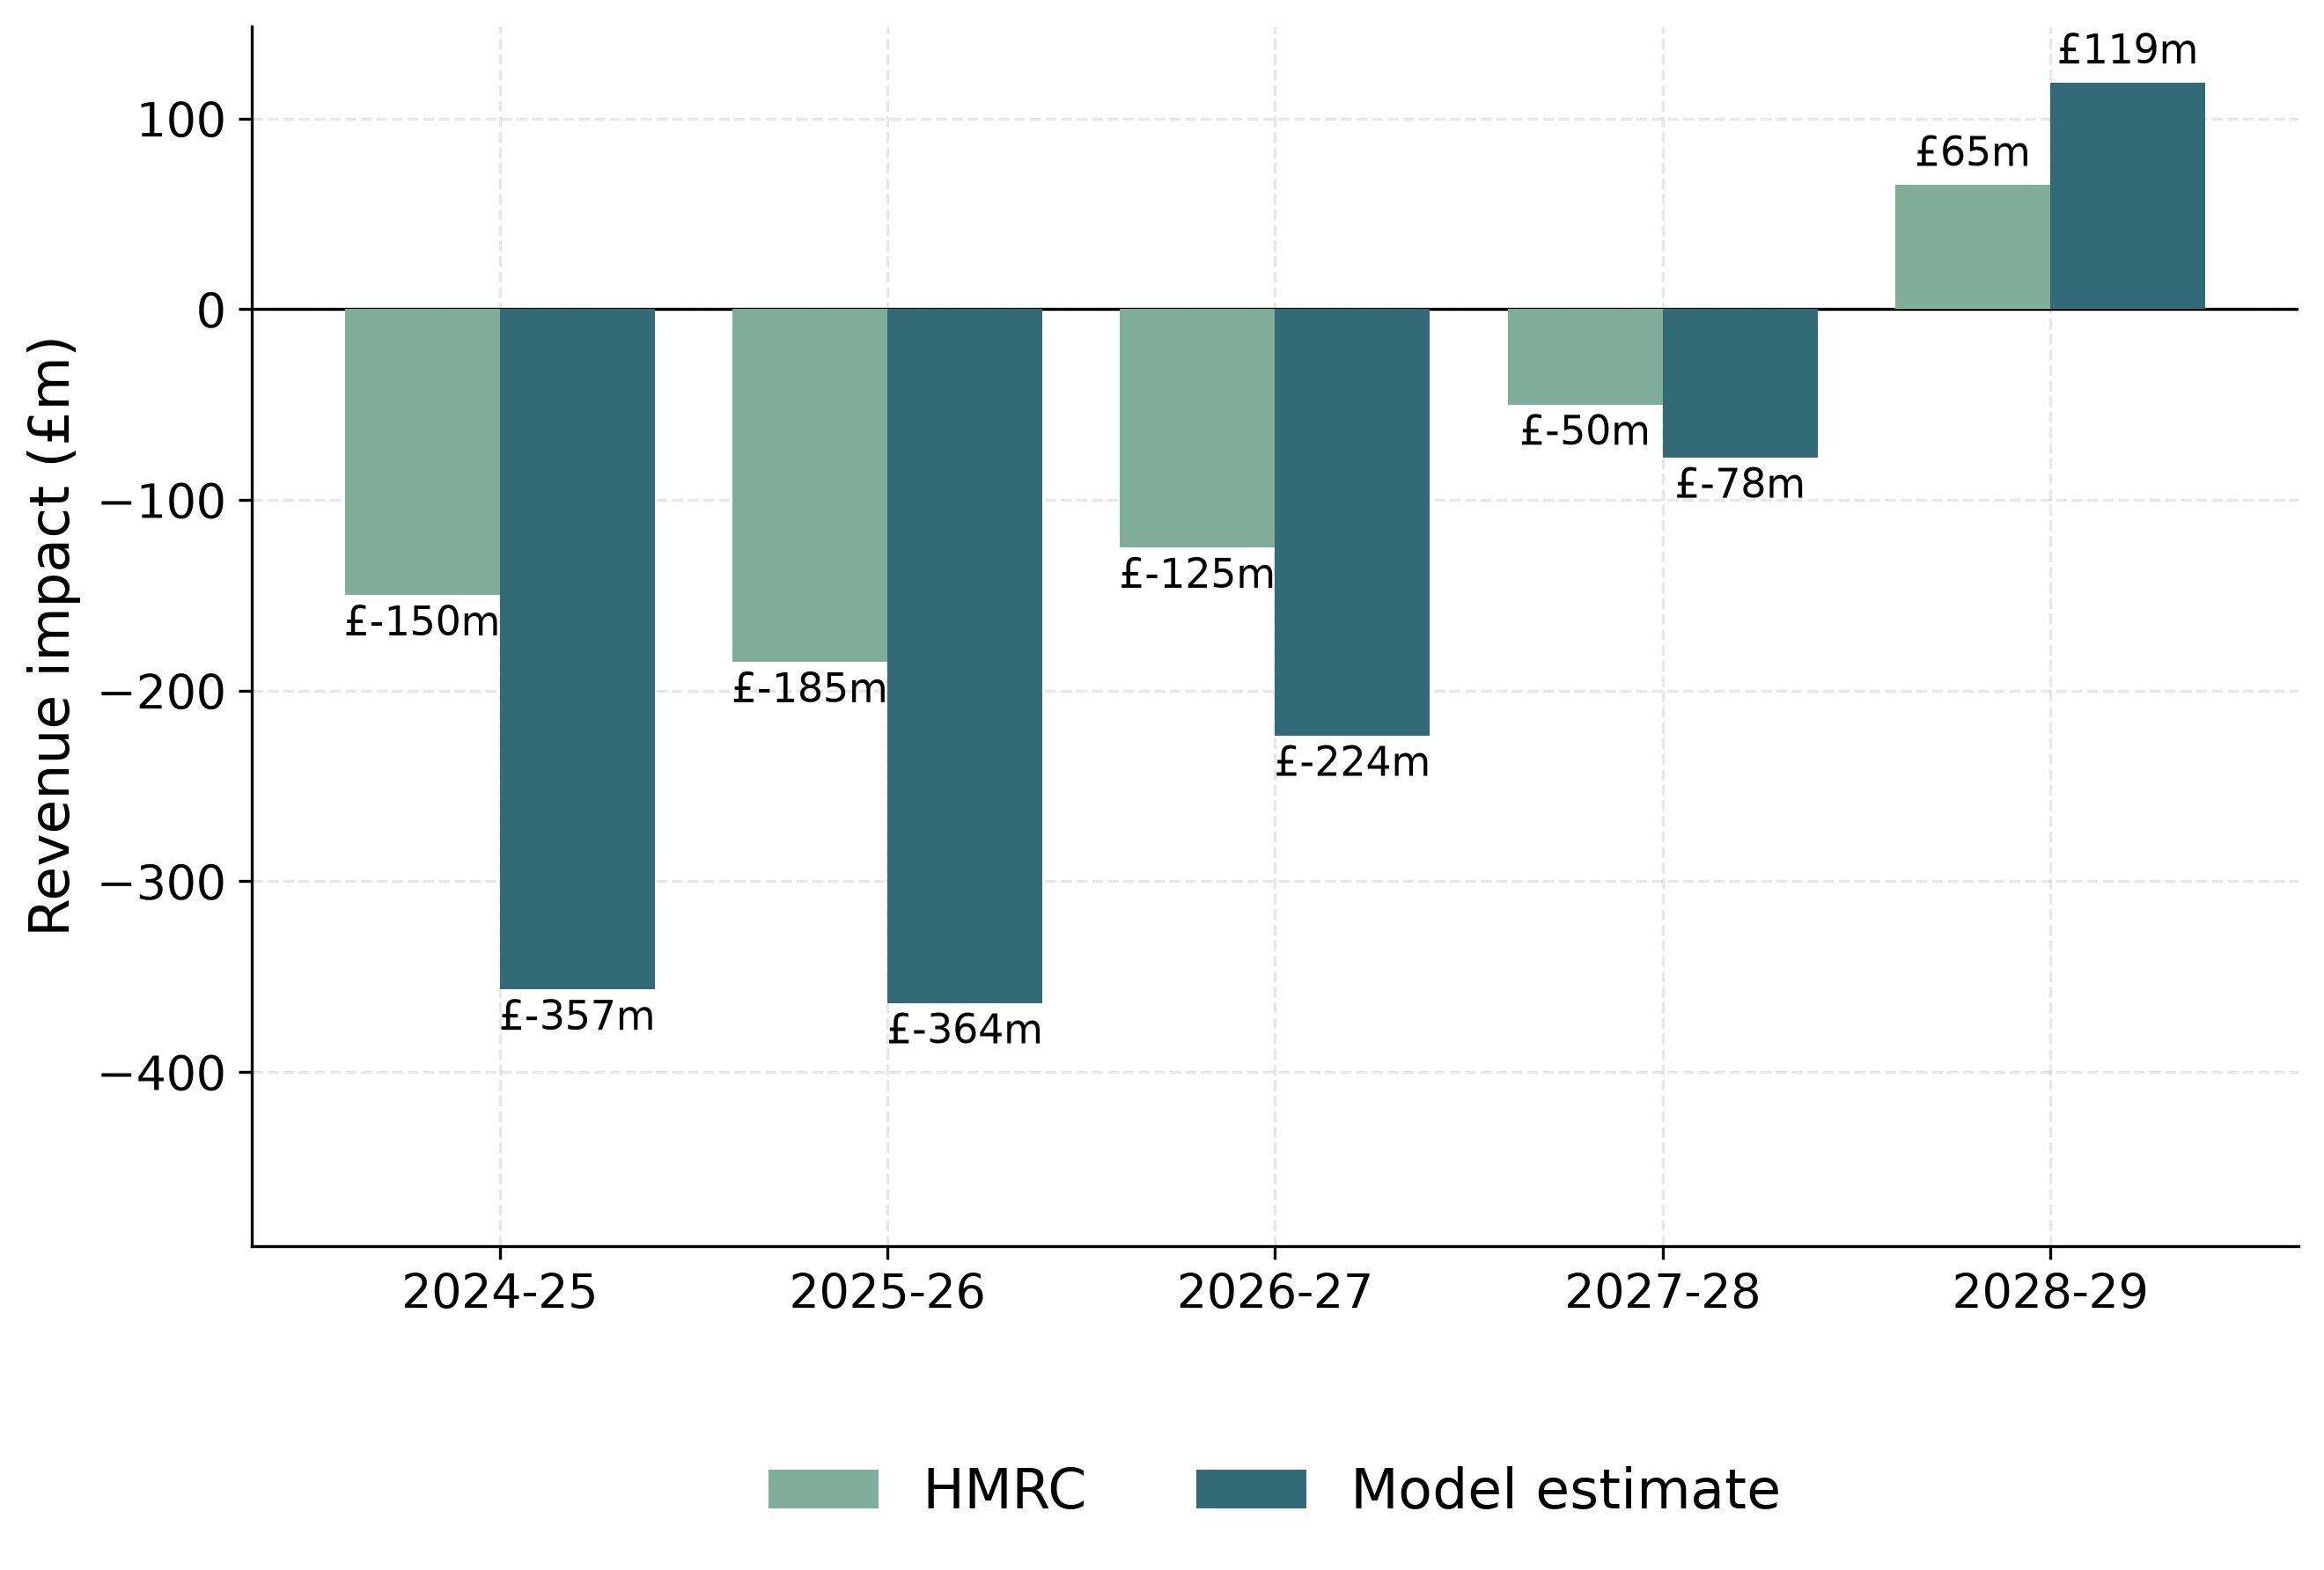
\includegraphics[width=0.78\textwidth]{figures/vat_threshold_revenue_impact.png}
\caption{Anchor reform: revenue impact of raising the VAT registration threshold
from \pounds85{,}000 to \pounds90{,}000 (the April~2024 change), my estimate
under the full-deregistration and 43\% retention conventions versus HMRC's
published costing, 2024--25 to 2028--29. Both series narrow over the
forecast and turn positive by 2028--29 because the costing baseline is a
counterfactual threshold path that resumes uprating after March~2026 and
overtakes \pounds90{,}000. The mechanical estimate, with no retention or
behavioural parameter, lies within 30\% of the official profile in each of
the four release years (within 10\% in 2025--26 and 2026--27) and 36\%
above it in the sign-flip year; the 43\% retention
convention undershoots it. Because the microdata are calibrated
to HMRC and OBR aggregates, this is a consistency check, not an out-of-sample
validation.}
\label{fig:hmrc_validation}
\end{figure}

\paragraph{A menu of threshold locations.} I next cost a menu of further threshold
locations, taking the post-reform \pounds90{,}000 threshold as the baseline. This
sweep runs on the 2024--25 vintage population (Section~\ref{sec:data}). Each
row of Table~\ref{tab:static_revenue} costs a move of the threshold to a new
location for 2025--26 by the registration rule above, holding the data-year
turnover distribution fixed, so the revenue change reflects only the
reclassification of in-scope firms into or out of the VAT net. Because the
optimiser determines the within-band shape near the threshold
(Section~\ref{sec:data}), and because the 2024--25 vintage has no fine-band
targets, so that its density steps at the \pounds90{,}000 HMRC band edge
(Section~\ref{sec:bunching}), the $\pm\pounds5{,}000$ rows are conditional on
that synthetic within-band allocation. Lowering the threshold draws in
in-scope firms not already registered---mainly the unregistered stratum, whose
liability under registration is the standard rate on its value added---while
raising it releases registered firms in the vacated band. A \pounds20{,}000
cut to \pounds70{,}000 raises about \pounds1.59bn and brings about 246{,}000
businesses into the net---at the standard rate on their modelled value added,
about \pounds6{,}400 per business; crediting them instead at HMRC's average
net remittance per registered below-threshold trader (\pounds2{,}152 in
2023--24) gives \pounds530m. A \pounds30{,}000 rise to \pounds120{,}000 costs
about \pounds1.28bn, 0.69\% of the \pounds184.1bn base. The cut rows
credit the full standard-rate liability of newly covered businesses, with no allowance for the compliance
cost or the registration lag a lower threshold would impose on them, and they
inherit the unregistered stratum's assumed exponential size distribution, so
they are illustrations of a maintained assumption rather than costings; the
per-firm-remittance variant above is the lower reading.
Figure~\ref{fig:static_sweep}
shows the sweep graphically. These are \emph{static} results: they bound the
first-order fiscal effect of a threshold change but abstract from the
behavioural response of Section~\ref{sec:behavioural}.

\begin{table}[htbp]
\centering
\caption{Static revenue and VAT-paying-firm effects of moving the VAT registration
threshold, 2025--26, relative to the post-reform \pounds90{,}000 baseline
(in-scope above-threshold VAT base \pounds184.1bn; 2024--25 vintage population).
Figures are mechanical, holding data-year turnover fixed (no behavioural
response); in-scope firms only, including the unregistered stratum below the
threshold. Voluntary registrants are held registered. Cut rows credit the full
liability of newly covered businesses (see text). This sweep is distinct from the anchor reform of
Figure~\ref{fig:hmrc_validation}. The machine-readable table is
\texttt{results/static\_sweep.txt} in the replication repository.}
\label{tab:static_revenue}
\begin{tabular}{lrrr}
\toprule
Threshold & Revenue change (\pounds m) & Change (\%) & VAT-paying firms (000s) \\
\midrule
\pounds70{,}000 & $+1{,}587.0$ & $+0.86$ & $+246.3$ \\
\pounds75{,}000 & $+1{,}171.0$ & $+0.64$ & $+175.3$ \\
\pounds80{,}000 & $+764.9$ & $+0.42$ & $+110.9$ \\
\pounds85{,}000 & $+376.5$ & $+0.20$ & $+52.7$ \\
\pounds90{,}000 (baseline) & $0$ & $0$ & $0$ \\
\pounds95{,}000 & $-198.0$ & $-0.11$ & $-28.8$ \\
\pounds100{,}000 & $-404.4$ & $-0.22$ & $-57.4$ \\
\pounds105{,}000 & $-625.9$ & $-0.34$ & $-86.3$ \\
\pounds110{,}000 & $-845.6$ & $-0.46$ & $-113.7$ \\
\pounds115{,}000 & $-1{,}066.0$ & $-0.58$ & $-139.6$ \\
\pounds120{,}000 & $-1{,}278.7$ & $-0.69$ & $-163.2$ \\
\bottomrule
\end{tabular}
\end{table}

\begin{figure}[htbp]
\centering
\subfigure[Revenue impact (\pounds m)]{%
    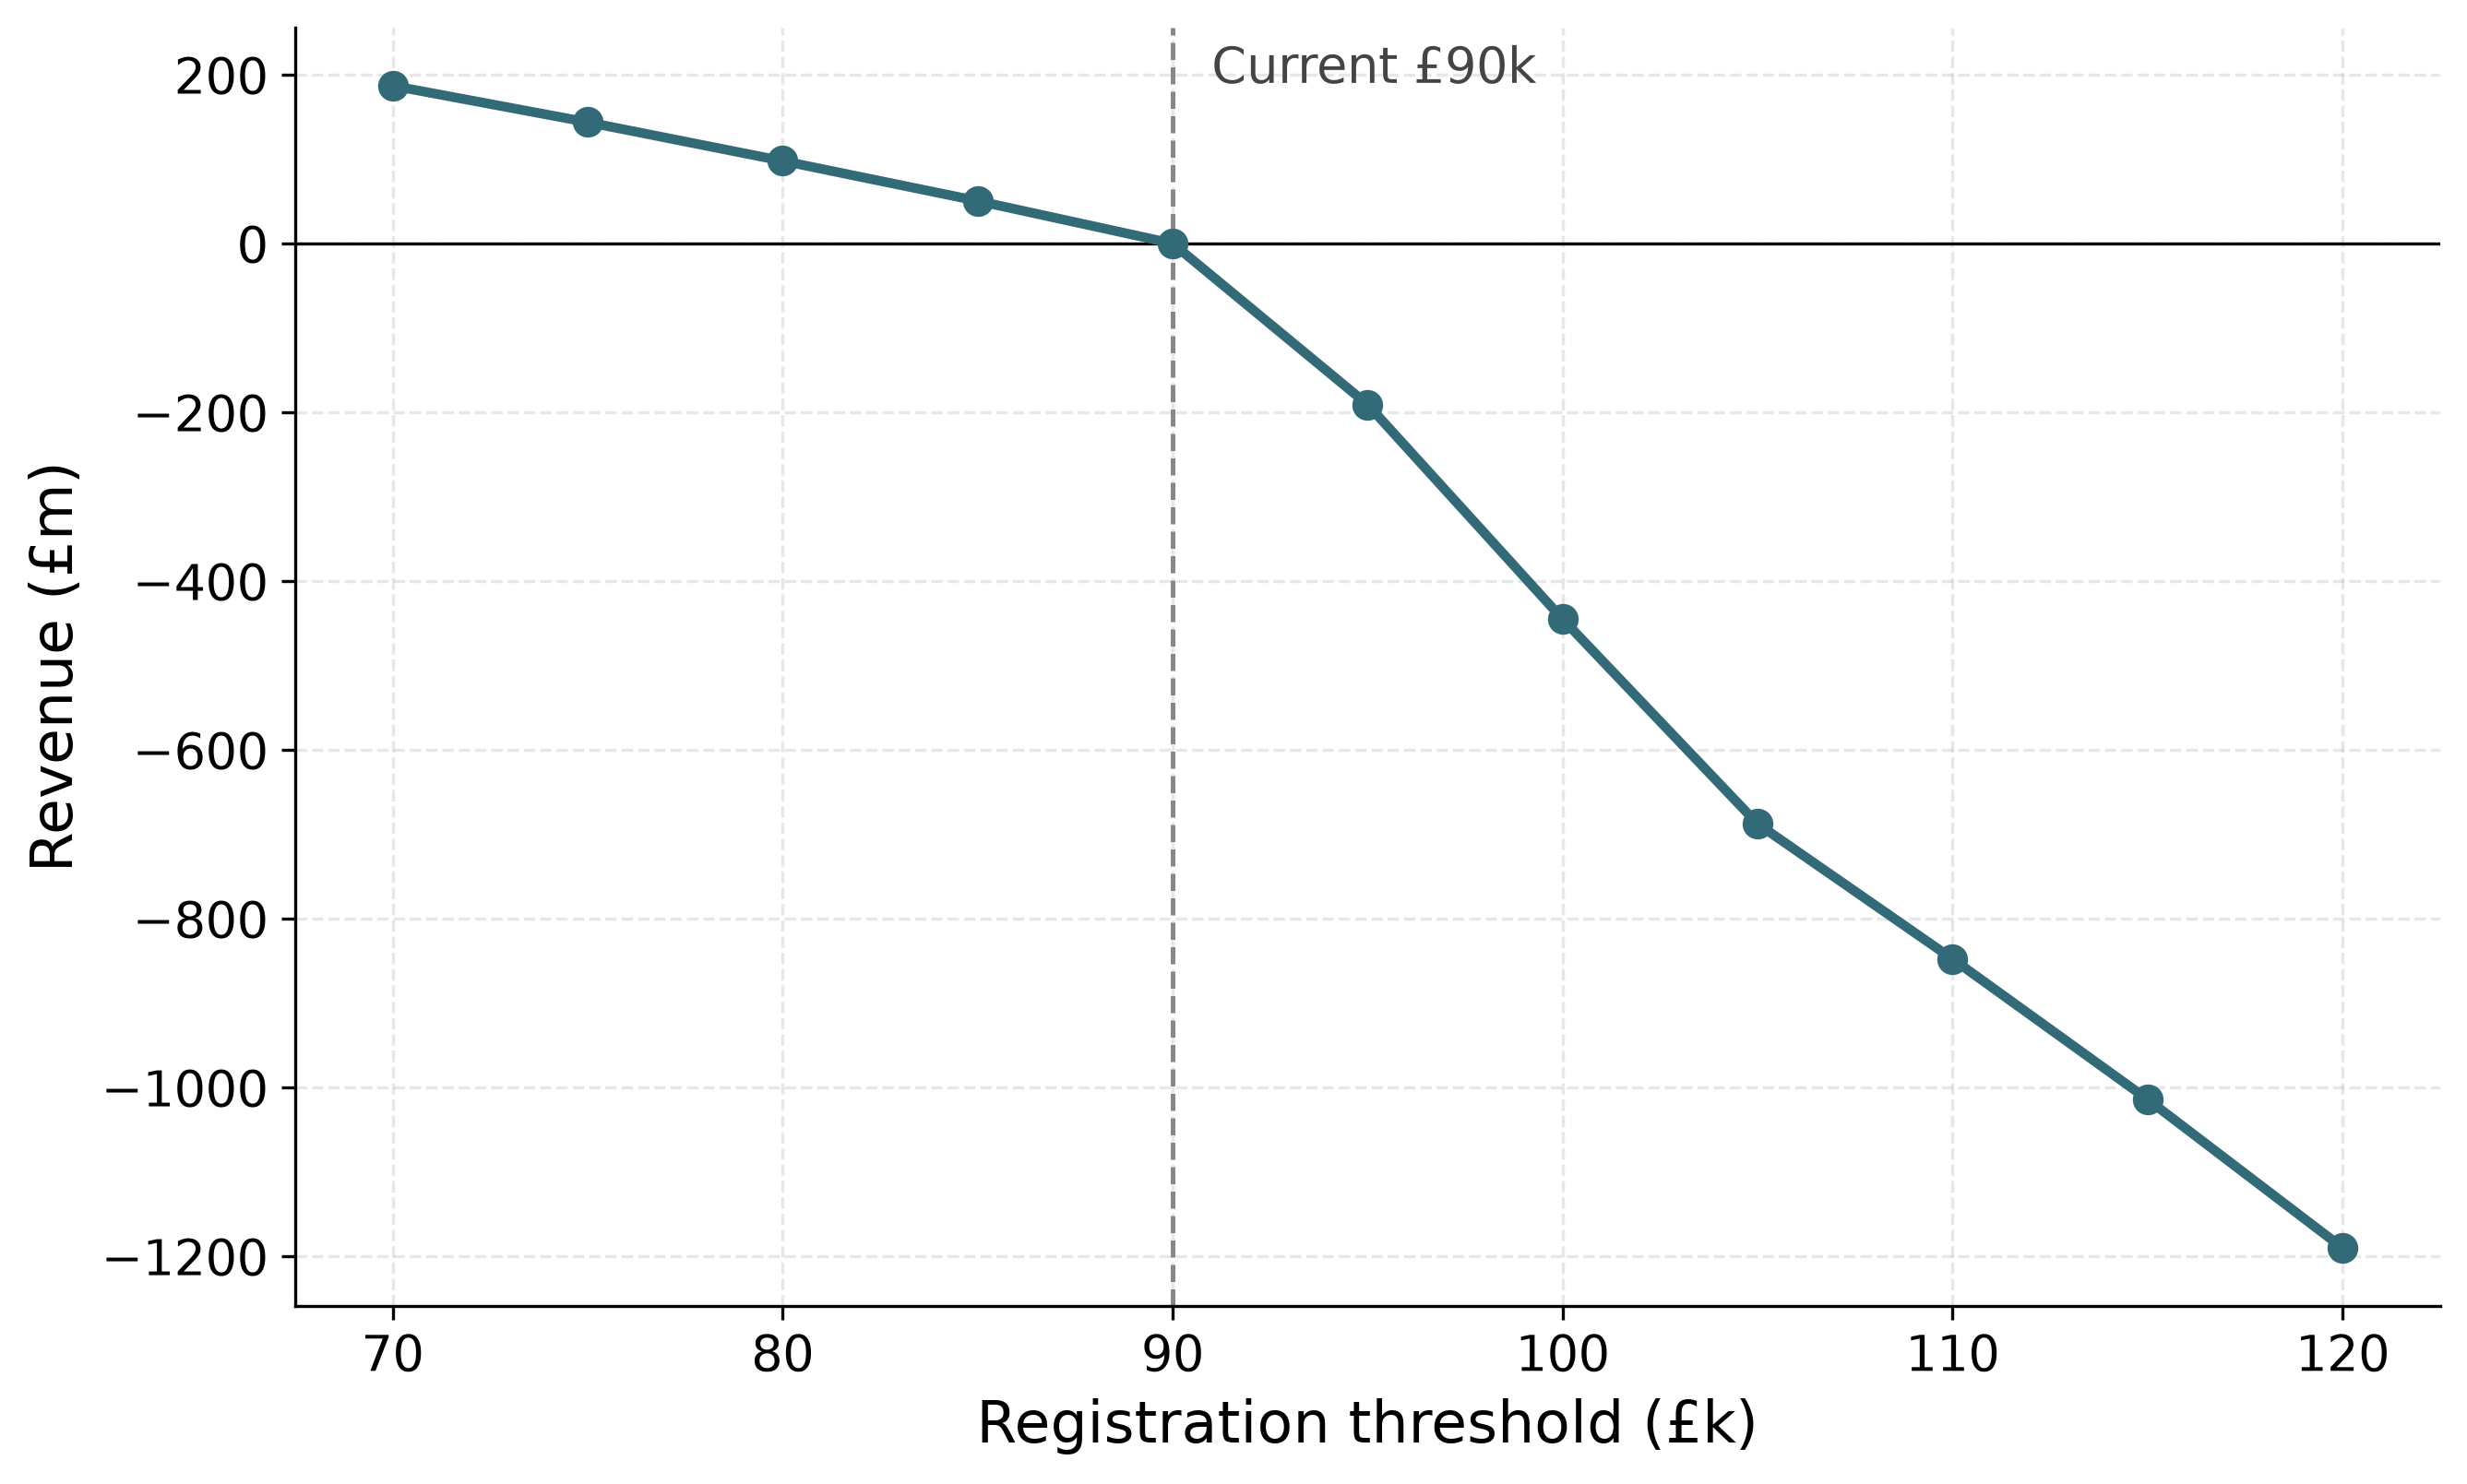
\includegraphics[width=0.48\textwidth]{figures/revenue_impact_2025_26.png}%
}\hfill%
\subfigure[Change in VAT-paying firms (000s)]{%
    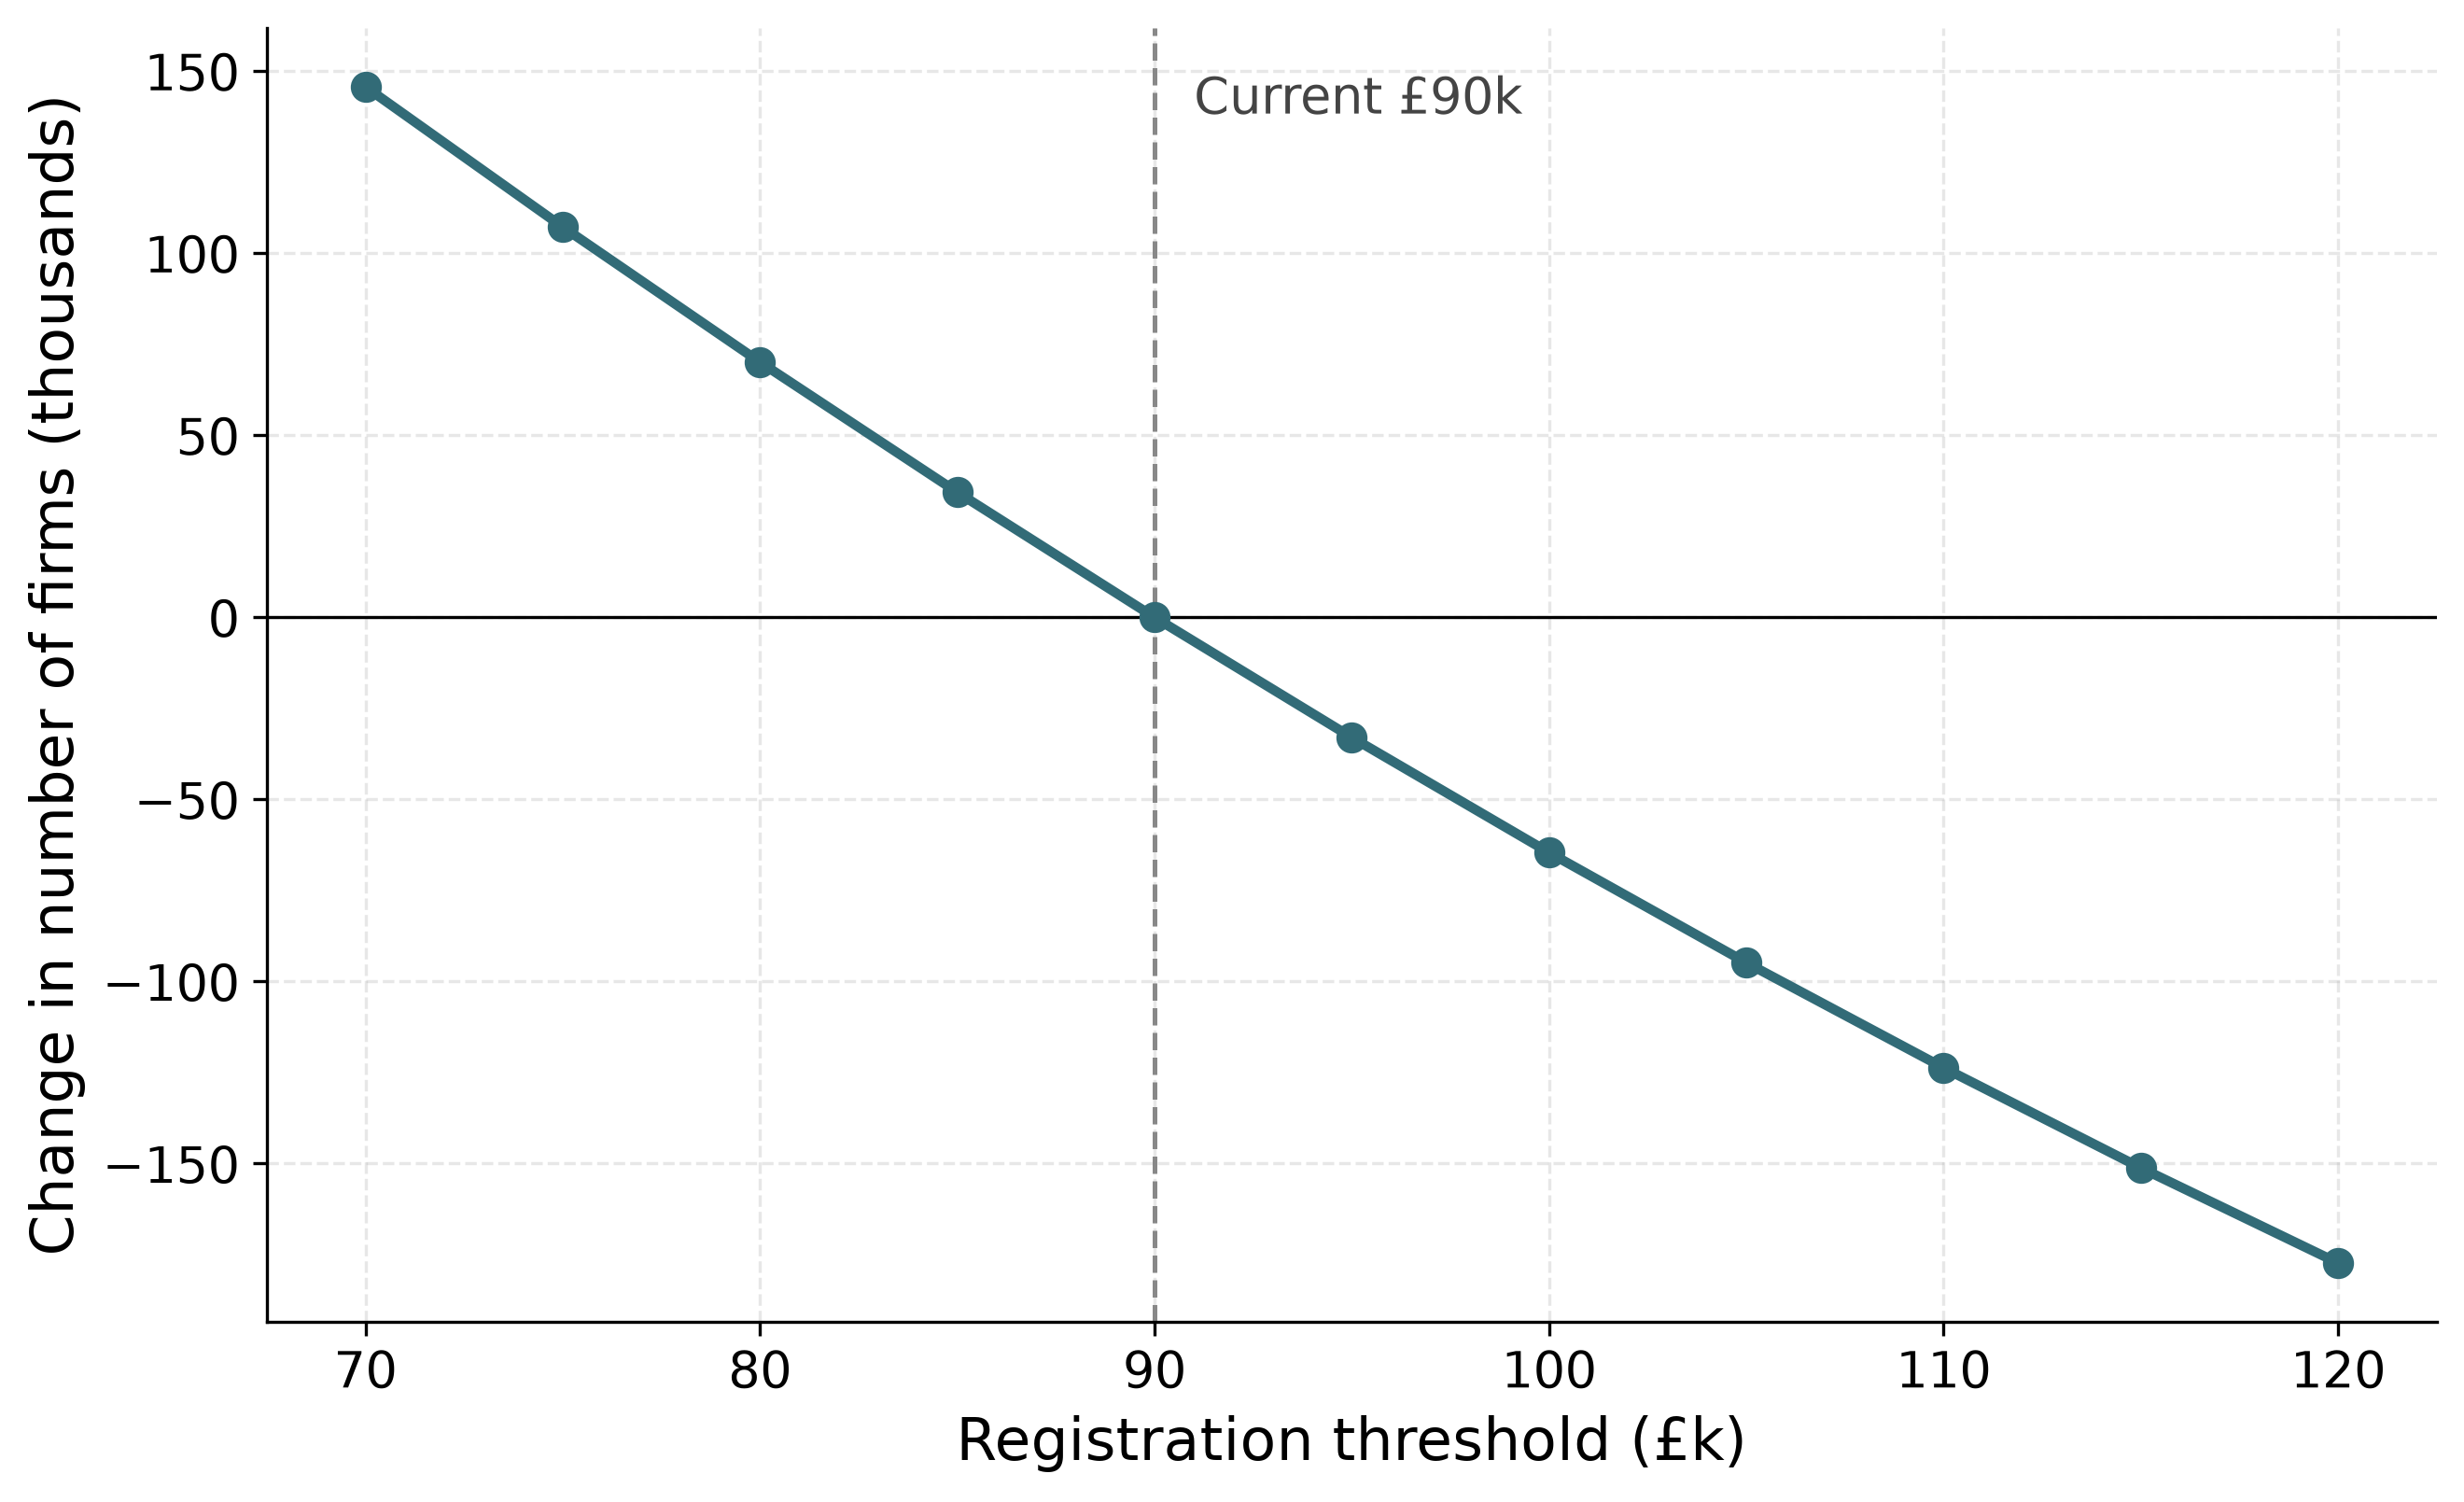
\includegraphics[width=0.48\textwidth]{figures/firms_impact_2025_26.png}%
}
\caption{Static effect of moving the VAT registration threshold, 2025--26, relative
to the \pounds90{,}000 baseline (dashed line). Panel (a): revenue impact---cuts
draw the unregistered stratum into the net; rises release registered firms.
Panel (b): the change in the
number of VAT-paying firms, tracking the local density of firms on each side of
the threshold.}
\label{fig:static_sweep}
\end{figure}

\subsection{Costing schedule reforms}
\label{ssec:schedule_costs}

The threshold sweep above moves the \emph{location} of a single cutoff. The same
static principle---re-applying a tax rule to the fixed turnover distribution, with
no behavioural response---also costs reforms that change the \emph{shape} of the
schedule rather than merely its position. I consider four reforms and report
their first-order revenue effects against a common baseline: the
\pounds85{,}000-notch / \pounds174.7bn 2023--24 base of in-scope firms. (This
2023--24 data-year base differs from the \pounds184.1bn figure in the sweep above, which runs on the
2024--25 vintage aged to 2025--26 at the post-reform \pounds90{,}000 threshold;
the schedule reforms are costed in the data year to match the bunching and
dominated-region analysis. Both bases are theoretical-liability (VTTL-style)
aggregates in the sense of the footnote above, not cash-receipts lines.) For each
reform I recompute the weighted sum of liabilities $R = \sum_i w_i\, v_i$ under
the new schedule, holding each firm's turnover fixed, and difference it against
the baseline.

\paragraph{Threshold relocation.} Raising the threshold from \pounds85{,}000 to
\pounds100{,}000 releases the firms with turnover in
$[\pounds85{,}000, \pounds100{,}000)$---about 87{,}800 in-scope
firms---from the VAT net, for a static revenue change of \(-\)\pounds583m on the
common base (the menu applies each schedule to in-scope firms at their data-year
turnover, without the deregistration-gap convention of the anchor). Because the
released band lies \emph{above} the data-year threshold, its liabilities are
directly calibrated (and its lower reach pinned by the OBR fine-band targets),
so the band is summed directly; a smooth-counterfactual alternative that fits
the above-threshold per-\pounds1{,}000 profile and integrates it across the
band gives \(-\)\pounds615m and 90{,}500 firms---within 6\% of the direct
sum now that the within-band fill is monotone. On this
common base the level move relocates the dominated region to the new cutoff and
widens it to \pounds25{,}000 (Section~\ref{sec:model}) at a static cost of
\(-\)\pounds583m; the linear taper removes the dominated region entirely at the
menu's largest static cost of \(-\)\pounds1{,}408m, and a constant-marginal-rate taper of
the same width does so at \(-\)\pounds932m (Section~\ref{sec:model}). Which matters more depends on what the
reader wants from the reform---the dominated-region metric indexes
misallocation only, and Section~\ref{sec:conclusion} discusses what it omits.

\paragraph{Graduated taper.} A graduated taper replaces the discrete notch with a
\emph{marginal} remittance rate that phases in over a band, so liability is the
integral of the marginal rate and a firm's \emph{effective} rate rises
continuously from $0\%$ to the full $20\%$ across the band. The band top is a
property of the chosen shape (Section~\ref{sec:model}): a taper whose marginal
rate is constant at $m>\tau$ meets the standard-rate line at
$U(m)=mT^{*}/(m-\tau)$, which is \pounds141{,}667 at $m=50\%$ and falls
towards \pounds106{,}250 as $m\to100\%$, while a taper reaching the full rate at
\pounds105{,}000 would push net revenue inside the band below its value at the
threshold, recreating a dominated interval smoothly rather than at a cliff. I
cost two designs on the same \pounds85{,}000--\pounds141{,}667 band: the
\emph{linear} taper, whose marginal rate rises from $0\%$ to $100\%$ across the
band, and a \emph{constant} $50\%$ marginal-rate taper. Firms in the band remit
the tapered schedule on their (fixed) turnover; mechanically the linear design
reduces revenue by \(-\)\pounds1{,}408m and the constant-rate design by \(-\)\pounds932m, with
about 278{,}100 in-scope firms in the band facing a lower effective rate.
The linear design gives more relief low in the band at the price of a marginal
remittance rate that reaches $100\%$ at the top; the constant-rate design caps
the marginal rate at $50\%$ and costs a third less.

\paragraph{Banded reduced rate.} A banded reduced rate charges firms in the
\pounds85{,}000--\pounds105{,}000 band a reduced rate
$\tau_{\text{low}}\in\{10\%,15\%\}$ in place of the standard $20\%$, with $20\%$
retained above \pounds105{,}000. Statically this reduces revenue by \(-\)\pounds398m
at $\tau_{\text{low}}=10\%$ and by \(-\)\pounds199m at $\tau_{\text{low}}=15\%$,
with about 117{,}300 in-scope firms in the band facing the lower rate.

\begin{table}[htbp]
\centering
\caption{Static, behaviour-free revenue effect of the reforms relative to the
common \pounds85{,}000-notch / \pounds174.7bn 2023--24 baseline of in-scope
firms. Each reform is costed mechanically by re-applying its schedule to the
fixed turnover distribution, with no behavioural response.}
\label{tab:schedule_costs}
\small
\begin{tabularx}{\textwidth}{@{}Xlr@{}}
\toprule
Reform & Lever & Static (\pounds m) \\
\midrule
Raise threshold to \pounds100{,}000 & Location & $-583$ \\
Linear taper, \pounds85k--\pounds141.7k & Shape (marginal rate $0\to100\%$) & $-1{,}408$ \\
Constant $50\%$ marginal taper, \pounds85k--\pounds141.7k & Shape (marginal rate $50\%$) & $-932$ \\
Reduced rate $10\%$, \pounds85k--\pounds105k & Rate (step) & $-398$ \\
Reduced rate $15\%$, \pounds85k--\pounds105k & Rate (step) & $-199$ \\
\bottomrule
\end{tabularx}
\end{table}

These static figures bound the first-order fiscal effect of each reform but
abstract from the behavioural response of Section~\ref{sec:behavioural}. Two
maintained conventions carry through every costing: the firm bears the full
statutory rate on its value added (no pass-through to prices), and per-firm
liability is the standard rate on value added, so Flat Rate Scheme users---who
are concentrated in exactly the \pounds85{,}000--\pounds150{,}000 bands---are
represented only through the calibrated band totals, not individually. One feature
of the shape reforms is not visible in a static costing: unlike a threshold move,
which transports the notch to a new cutoff, the taper and the reduced rate
\emph{change the size of the notch itself}---the discrete drop in net revenue at the
threshold and the empty band of turnover it induces. Quantifying that change
requires the structural object I develop in Section~\ref{sec:model}, where I derive
the notch's dominated region and show analytically how each of these reforms alters
it.
